\paragraph{QuizziPedia::Front-End::Controllers::AppController}
\begin{figure} [ht]
	\centering
	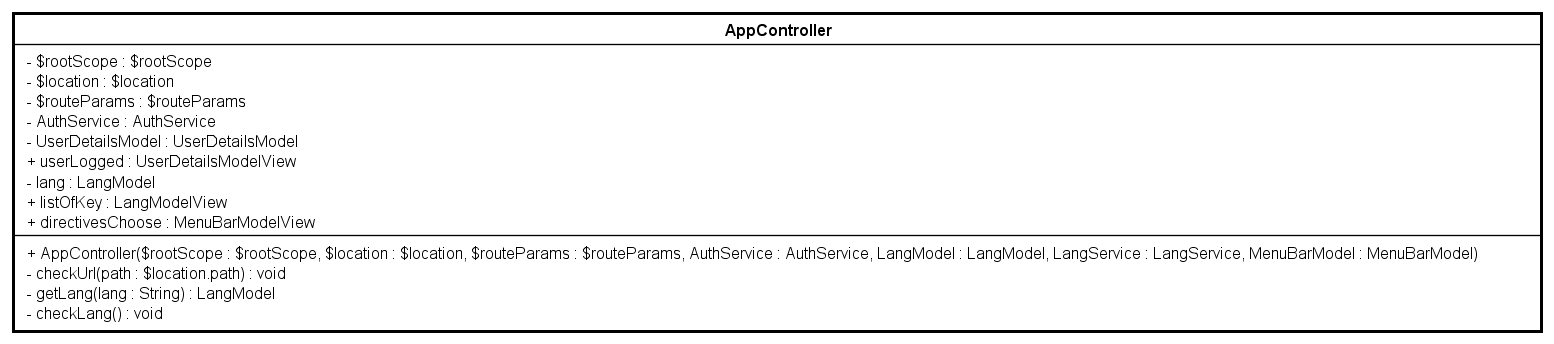
\includegraphics[scale=0.35]{UML/Classi/Front-End/QuizziPedia_Front-end_Controller_AppController.png}
	\caption{QuizziPedia::Front-End::Controllers::AppController}
\end{figure} \FloatBarrier
\begin{itemize}
	\item \textbf{Descrizione}: questa classe permette di gestire per ogni pagina dell'applicazione l'autenticazione e l'autorizzazione dell'utente che si posiziona in essa e mostrare la lingua corretta;
	\item \textbf{Utilizzo}: fornisce le funzionalità per gestire per ogni pagina dell'applicazione l'autenticazione e l'autorizzazione dell'utente che si posiziona in essa e mostrare la lingua corretta;
	\item \textbf{Relazione con altre classi}:
	\begin{itemize}
		\item \textbf{IN \texttt{UserDetailsModelView}}: classe di tipo \textit{modelview\ped{G}} la cui istanziazione è contenuta all'interno della variabile di ambiente \$rootScope di \textit{Angular\ped{G}}. All'interno di essa sono presenti le variabili e i metodi necessari per il \textit{Two-Way Data-Binding\ped{G}} tra le \textit{views\ped{G}} e i \textit{controllers\ped{G}} che necessitano di utilizzare l'utente autenticato;
		\item \textbf{IN \texttt{UserDetailsModel}}: rappresenta un utente. Contiene tutte le informazioni necessarie alla presentazione del contenuto di un utente sia nella visualizzazione che nella gestione di un profilo;
		\item \textbf{IN} \texttt{LangService}: questa classe permette di gestire la lingua nella quale si è scelto di utilizzare l'applicazione;
		\item \textbf{IN} \texttt{LangModel}: rappresenta le informazioni per la giusta traduzione dell'applicazione;
		\item \textbf{IN} \texttt{AuthService}: questa classe permette di gestire la registrazione e l'autenticazione di un utente;
		\item \textbf{IN} \texttt{MenuBarModel}: questa classe rappresenta la classe che contiene le informazioni per la giusta visualizzazione della barra;
		\item \textbf{IN} \texttt{MenuBarModelView}: classe di tipo modelview la cui istanziazione è contenuta all'interno della variabile di ambiente \texttt{\$rootScope} di \textit{Angular\ped{G}}. All'interno di essa sono presenti le variabili e i metodi necessari per il \textit{Two-Way Data-Binding\ped{G}} tra la \textit{view\ped{G}} \texttt{Index} e il \textit{controller\ped{G}} \texttt{MenuBarController};
		\item \textbf{OUT} \texttt{AppRouter}: classe che gestisce i routes dell’applicazione, utilizza il servizio \texttt{\$routeProvider} per associare ad ogni route un \textit{controller\ped{G}} e una \textit{view\ped{G}}. \texttt{Appcontroller} viene chiamato ogni volta che \texttt{AppRouter} instrada una vista.
	\end{itemize}
	\item \textbf{Attributi}:
	\begin{itemize}
		\item \texttt{-} \texttt{\$rootScope: \$rootScope} \\
		Campo dati contenente il riferimento all'oggetto globale \$rootScope creato da \textit{Angular\ped{G}}. Viene utilizzato per rendere accessibile a tutti i \textit{controller\ped{G}} e a tutte le \textit{view\ped{G}} l'oggetto \texttt{UserDetailsModel};
		\item \texttt{-} \texttt{\$location: \$location} \\
		Campo dati contenente un riferimento al servizio creato da \textit{Angular\ped{G}} che permette di accedere alla barra degli indirizzi del \textit{browser\ped{G}}, i cambiamenti all'URL nella barra degli indirizzi si riflettono in questo oggetto e viceversa; 
		\item \texttt{-} \texttt{\$routeParams: \$routeParams} \\
		Campo dati contenente il riferimento all'oggetto globale \$routeParams creato da \textit{Angular\ped{G}}. Tale servizio permette di recuperare il set di variabili presenti nell'url;
		\item \texttt{-} \texttt{UserDetailsModel: UserDetailsModel} \\
		Campo dati contenente un riferimento alla classe per poter istanziare un oggetto di tipo \texttt{UserDetailsModel};
		\item \texttt{-} \texttt{AuthService: AuthService} \\
		Campo dati contenente un riferimento al servizio che si occupa della gestione delle informazioni legate all’autenticazione;
		\item \texttt{-} \texttt{LangModel: LangModel} \\
		Campo dati contenente un riferimento alla classe rappresenta le informazioni per la giusta traduzione dell'applicazione;
		\item \texttt{-} \texttt{LangService: LangService} \\
		Campo dati contenente un riferimento alla classe che permette di gestire la lingua nella quale si è scelto di utilizzare l'applicazione;
		\item \texttt{-} \texttt{directivesChoose: MenuBarModelView}: \\
		Campo dati contenente un oggetto di tipo modelview la cui istanziazione è contenuta all'interno della variabile di ambiente \texttt{\$rootScope} di \textit{Angular\ped{G}}. All'interno di essa sono presenti le variabili e i metodi necessari per il \textit{Two-Way Data-Binding\ped{G}} tra la \textit{view\ped{G}} \texttt{Index} e il \textit{controller\ped{G}} \texttt{MenuBarController}. Rappresenta un oggetto di tipo \texttt{MenuBarModel};
		\item \texttt{+} \texttt{systemLang: String} \\
		Campo dati contenente una stringa in cui viene memorizzata la lingua del sistama;
		\item \texttt{+} \texttt{listOfKeys: LangModelView}\\ 
		Classe di tipo \textit{modelview\ped{G}} la cui istanziazione è contenuta all'interno della variabile di ambiente \$rootScope di \textit{Angular\ped{G}}. All'interno di essa sono presenti le variabili e i metodi necessari per il \textit{Two-Way Data-Binding\ped{G}} tra le \textit{views\ped{G}} e i \textit{controllers\ped{G}} per la visualizzazione nella lingua corretta dell'applicazione;
		\item \texttt{+} \texttt{userLogged: UserDetailsModelView} \\
		Oggetto di tipo \texttt{UserDetailsModelView}. All'interno di essa sono presenti le variabili e i metodi necessari per il \textit{Two-Way Data-Binding\ped{G}} tra le \textit{views\ped{G}} e i \textit{controllers\ped{G}} che necessitano di utilizzare l'utente autenticato. Rappresenta nello \$rootScope un oggetto di tipo \texttt{UserDetailsModel}.
	\end{itemize}	
		\item \textbf{Metodi}:
		\begin{itemize}
		\item \texttt{+} \texttt{AppController (\$rootScope: \$rootScope, \$location: \$location, \$routeParams: \$routeParams, UserDetailsModel: UserDetailsModel, AuthService: AuthService, LangModel: LangModel, LangService: LangService, MenuBarModel: MenuBarModel )} \\ Metodo costruttore della classe. Una volta che viene creato l'oggetto esso esegue tutte le operazioni possibili per capire il livello di autorizzazione e di scaricare la giusta lingua per l'applicazione.\\
		\textbf{Parametri}: 
		\begin{itemize}
			\item \texttt{\$rootScope: \$rootScope} \\
			Parametro contenente il riferimento all'oggetto globale \$rootScope creato da \textit{An-\\gular\ped{G}}. Viene utilizzato per rendere accessibile a tutti i \textit{controller\ped{G}} e a tutte le \textit{view\ped{G}} l'oggetto \texttt{UserDetailsModel}. In questo caso viene utilizzato per inserire in \$rootScope l'oggetto di ritorno della chiamata a \texttt{getUserDetails} del \textit{service\ped{G}} \texttt{UserDetai-\\lsService};
			\item \texttt{-} \texttt{\$location: \$location} \\
			Campo dati contenente un riferimento al servizio creato da \textit{Angular\ped{G}} che permette di accedere alla barra degli indirizzi del \textit{browser\ped{G}}, i cambiamenti all'URL nella barra degli indirizzi si riflettono in questo oggetto e viceversa; 
			\item \texttt{\$routeParams: \$routeParams} \\
			Campo dati contenente il riferimento all'oggetto globale \$routeParams creato da \textit{Angular\ped{G}}. Tale servizio permette di recuperare il set di variabili presenti nell'url.
			\item \texttt{UserDetailsModel: UserDetailsModel} \\
			Parametro contenente un riferimento alla classe per poter istanziare un oggetto di tipo \texttt{UserDetailsModel};
			\item \texttt{AuthService: AuthService} \\
			Parametro contenente un riferimento al servizio che si occupa della gestione delle informazioni legate all’autenticazione;
			\item \texttt{LangModel: LangModel} \\
			Parametro contenente un riferimento alla classe rappresenta le informazioni per la giusta traduzione dell'applicazione;;
			\item \texttt{LangService: LangService} \\
			Parametro contenente un riferimento alla classe che permette di gestire la lingua nella quale si è scelto di utilizzare l'applicazione
			\item \texttt{MenuBarModel: MenuBarModel}: \\
			Parametro contenente un riferimento all'oggetto che contiene le informazioni per la giusta visualizzazione della barra.
		\end{itemize}
		\item \texttt{-} \texttt{getLang(lang: String): LangModel} \\ Metodo che permette di ottenere i dati con una chiamata a \texttt{LangService}.\\
		\textbf{Parametri}:
		\begin{itemize}
			\item \texttt{lang: String}: parametro che identifica la lingua del sistema.
		\end{itemize}
		\item \texttt{-} \texttt{checkUrl(lang: \$location.path): void} \\ Metodo che gestisce l'autorizzazione dell'utente nella pagina in cui si trova;
		\item \texttt{-} \texttt{checkLang(): void} \\ Metodo che controlla se la lingua presente nell'url sia tra una di quelle supportate dal sistema.
	\end{itemize}
\end{itemize}

